% Options for packages loaded elsewhere
\PassOptionsToPackage{unicode}{hyperref}
\PassOptionsToPackage{hyphens}{url}
%
\documentclass[
]{article}
\usepackage{amsmath,amssymb}
\usepackage{iftex}
\ifPDFTeX
  \usepackage[T1]{fontenc}
  \usepackage[utf8]{inputenc}
  \usepackage{textcomp} % provide euro and other symbols
\else % if luatex or xetex
  \usepackage{unicode-math} % this also loads fontspec
  \defaultfontfeatures{Scale=MatchLowercase}
  \defaultfontfeatures[\rmfamily]{Ligatures=TeX,Scale=1}
\fi
\usepackage{lmodern}
\ifPDFTeX\else
  % xetex/luatex font selection
\fi
% Use upquote if available, for straight quotes in verbatim environments
\IfFileExists{upquote.sty}{\usepackage{upquote}}{}
\IfFileExists{microtype.sty}{% use microtype if available
  \usepackage[]{microtype}
  \UseMicrotypeSet[protrusion]{basicmath} % disable protrusion for tt fonts
}{}
\makeatletter
\@ifundefined{KOMAClassName}{% if non-KOMA class
  \IfFileExists{parskip.sty}{%
    \usepackage{parskip}
  }{% else
    \setlength{\parindent}{0pt}
    \setlength{\parskip}{6pt plus 2pt minus 1pt}}
}{% if KOMA class
  \KOMAoptions{parskip=half}}
\makeatother
\usepackage{xcolor}
\usepackage[margin=1in]{geometry}
\usepackage{color}
\usepackage{fancyvrb}
\newcommand{\VerbBar}{|}
\newcommand{\VERB}{\Verb[commandchars=\\\{\}]}
\DefineVerbatimEnvironment{Highlighting}{Verbatim}{commandchars=\\\{\}}
% Add ',fontsize=\small' for more characters per line
\usepackage{framed}
\definecolor{shadecolor}{RGB}{248,248,248}
\newenvironment{Shaded}{\begin{snugshade}}{\end{snugshade}}
\newcommand{\AlertTok}[1]{\textcolor[rgb]{0.94,0.16,0.16}{#1}}
\newcommand{\AnnotationTok}[1]{\textcolor[rgb]{0.56,0.35,0.01}{\textbf{\textit{#1}}}}
\newcommand{\AttributeTok}[1]{\textcolor[rgb]{0.13,0.29,0.53}{#1}}
\newcommand{\BaseNTok}[1]{\textcolor[rgb]{0.00,0.00,0.81}{#1}}
\newcommand{\BuiltInTok}[1]{#1}
\newcommand{\CharTok}[1]{\textcolor[rgb]{0.31,0.60,0.02}{#1}}
\newcommand{\CommentTok}[1]{\textcolor[rgb]{0.56,0.35,0.01}{\textit{#1}}}
\newcommand{\CommentVarTok}[1]{\textcolor[rgb]{0.56,0.35,0.01}{\textbf{\textit{#1}}}}
\newcommand{\ConstantTok}[1]{\textcolor[rgb]{0.56,0.35,0.01}{#1}}
\newcommand{\ControlFlowTok}[1]{\textcolor[rgb]{0.13,0.29,0.53}{\textbf{#1}}}
\newcommand{\DataTypeTok}[1]{\textcolor[rgb]{0.13,0.29,0.53}{#1}}
\newcommand{\DecValTok}[1]{\textcolor[rgb]{0.00,0.00,0.81}{#1}}
\newcommand{\DocumentationTok}[1]{\textcolor[rgb]{0.56,0.35,0.01}{\textbf{\textit{#1}}}}
\newcommand{\ErrorTok}[1]{\textcolor[rgb]{0.64,0.00,0.00}{\textbf{#1}}}
\newcommand{\ExtensionTok}[1]{#1}
\newcommand{\FloatTok}[1]{\textcolor[rgb]{0.00,0.00,0.81}{#1}}
\newcommand{\FunctionTok}[1]{\textcolor[rgb]{0.13,0.29,0.53}{\textbf{#1}}}
\newcommand{\ImportTok}[1]{#1}
\newcommand{\InformationTok}[1]{\textcolor[rgb]{0.56,0.35,0.01}{\textbf{\textit{#1}}}}
\newcommand{\KeywordTok}[1]{\textcolor[rgb]{0.13,0.29,0.53}{\textbf{#1}}}
\newcommand{\NormalTok}[1]{#1}
\newcommand{\OperatorTok}[1]{\textcolor[rgb]{0.81,0.36,0.00}{\textbf{#1}}}
\newcommand{\OtherTok}[1]{\textcolor[rgb]{0.56,0.35,0.01}{#1}}
\newcommand{\PreprocessorTok}[1]{\textcolor[rgb]{0.56,0.35,0.01}{\textit{#1}}}
\newcommand{\RegionMarkerTok}[1]{#1}
\newcommand{\SpecialCharTok}[1]{\textcolor[rgb]{0.81,0.36,0.00}{\textbf{#1}}}
\newcommand{\SpecialStringTok}[1]{\textcolor[rgb]{0.31,0.60,0.02}{#1}}
\newcommand{\StringTok}[1]{\textcolor[rgb]{0.31,0.60,0.02}{#1}}
\newcommand{\VariableTok}[1]{\textcolor[rgb]{0.00,0.00,0.00}{#1}}
\newcommand{\VerbatimStringTok}[1]{\textcolor[rgb]{0.31,0.60,0.02}{#1}}
\newcommand{\WarningTok}[1]{\textcolor[rgb]{0.56,0.35,0.01}{\textbf{\textit{#1}}}}
\usepackage{graphicx}
\makeatletter
\def\maxwidth{\ifdim\Gin@nat@width>\linewidth\linewidth\else\Gin@nat@width\fi}
\def\maxheight{\ifdim\Gin@nat@height>\textheight\textheight\else\Gin@nat@height\fi}
\makeatother
% Scale images if necessary, so that they will not overflow the page
% margins by default, and it is still possible to overwrite the defaults
% using explicit options in \includegraphics[width, height, ...]{}
\setkeys{Gin}{width=\maxwidth,height=\maxheight,keepaspectratio}
% Set default figure placement to htbp
\makeatletter
\def\fps@figure{htbp}
\makeatother
\setlength{\emergencystretch}{3em} % prevent overfull lines
\providecommand{\tightlist}{%
  \setlength{\itemsep}{0pt}\setlength{\parskip}{0pt}}
\setcounter{secnumdepth}{-\maxdimen} % remove section numbering
\ifLuaTeX
  \usepackage{selnolig}  % disable illegal ligatures
\fi
\usepackage{bookmark}
\IfFileExists{xurl.sty}{\usepackage{xurl}}{} % add URL line breaks if available
\urlstyle{same}
\hypersetup{
  pdftitle={DATA 405 Assignment 2},
  pdfauthor={Rin Meng 51940633},
  hidelinks,
  pdfcreator={LaTeX via pandoc}}

\title{DATA 405 Assignment 2}
\author{Rin Meng 51940633}
\date{}

\begin{document}
\maketitle

\section{Question 1}\label{question-1}

a).

\begin{Shaded}
\begin{Highlighting}[]
\NormalTok{X }\OtherTok{\textless{}{-}} \FunctionTok{c}\NormalTok{(}\FloatTok{0.5}\NormalTok{, }\FloatTok{0.3}\NormalTok{, }\FloatTok{0.2}\NormalTok{)}
\NormalTok{cumsum.X }\OtherTok{\textless{}{-}} \FunctionTok{cumsum}\NormalTok{(X)}
\NormalTok{cumsum.X}
\end{Highlighting}
\end{Shaded}

\begin{verbatim}
## [1] 0.5 0.8 1.0
\end{verbatim}

b).

\begin{Shaded}
\begin{Highlighting}[]
\NormalTok{pX }\OtherTok{\textless{}{-}} \ControlFlowTok{function}\NormalTok{ (x)\{}
  \FunctionTok{return}\NormalTok{(cumsum.X[x}\SpecialCharTok{+}\DecValTok{1}\NormalTok{])}
\NormalTok{\}}
\end{Highlighting}
\end{Shaded}

c).

\begin{Shaded}
\begin{Highlighting}[]
\NormalTok{rX }\OtherTok{\textless{}{-}} \ControlFlowTok{function}\NormalTok{(x)\{}
\NormalTok{  U }\OtherTok{\textless{}{-}} \FunctionTok{runif}\NormalTok{(x)}
\NormalTok{  X }\OtherTok{\textless{}{-}} \FunctionTok{numeric}\NormalTok{(x)}
\NormalTok{  x }\OtherTok{\textless{}{-}} \DecValTok{0}
  \ControlFlowTok{for}\NormalTok{ (x }\ControlFlowTok{in} \DecValTok{0}\SpecialCharTok{:}\DecValTok{6}\NormalTok{) \{}
\NormalTok{    X[U }\SpecialCharTok{\textgreater{}=} \FunctionTok{pX}\NormalTok{(x)] }\OtherTok{\textless{}{-}}\NormalTok{ x }\SpecialCharTok{+} \DecValTok{1}
\NormalTok{    x }\OtherTok{\textless{}{-}}\NormalTok{ x}\SpecialCharTok{+}\DecValTok{1}
\NormalTok{  \}}
  \FunctionTok{return}\NormalTok{(X)}
\NormalTok{\}}
\FunctionTok{rX}\NormalTok{(}\DecValTok{10}\NormalTok{)}
\end{Highlighting}
\end{Shaded}

\begin{verbatim}
##  [1] 2 2 1 0 1 0 0 1 2 1
\end{verbatim}

d).

\begin{Shaded}
\begin{Highlighting}[]
\NormalTok{myX }\OtherTok{\textless{}{-}} \FunctionTok{rX}\NormalTok{(}\DecValTok{1000}\NormalTok{)}
\end{Highlighting}
\end{Shaded}

e).

\begin{Shaded}
\begin{Highlighting}[]
\FunctionTok{table}\NormalTok{(myX)}
\end{Highlighting}
\end{Shaded}

\begin{verbatim}
## myX
##   0   1   2 
## 503 290 207
\end{verbatim}

No these values do not differ from what we would have expected, because
for \(n = 1000\), we can say that \(E[0] = 0.5 \times 1000 = 500\) and
\(E[1] = 0.3 \times 1000 = 300\) and also,
\(E[2] = 0.2 \times 1000 = 200\), where as our values observed, is
relatively close to those values.

f).

\begin{Shaded}
\begin{Highlighting}[]
\FunctionTok{barplot}\NormalTok{(}\FunctionTok{table}\NormalTok{(myX), }\AttributeTok{xlab =} \StringTok{"Probability of getting X = x"}\NormalTok{, }\AttributeTok{ylab=}\StringTok{"Occurance Frequency"}\NormalTok{,}\AttributeTok{ylim =} \FunctionTok{c}\NormalTok{(}\DecValTok{0}\NormalTok{,}\DecValTok{500}\NormalTok{), }\AttributeTok{main=}\StringTok{"Probability histogram"}\NormalTok{)}
\end{Highlighting}
\end{Shaded}

\begin{figure}
\centering
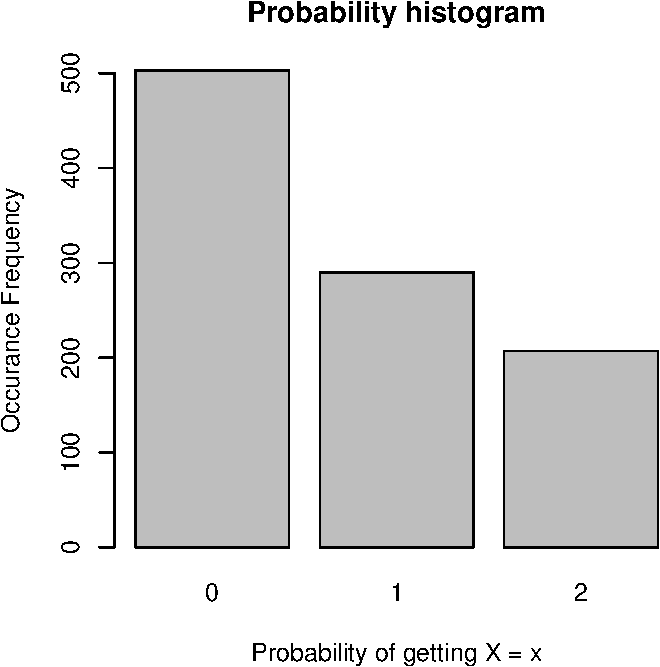
\includegraphics{a2_files/figure-latex/unnamed-chunk-6-1.pdf}
\caption{Probability histogram of myX}
\end{figure}

\section{Question 2}\label{question-2}

\begin{Shaded}
\begin{Highlighting}[]
\NormalTok{binsim }\OtherTok{\textless{}{-}} \FunctionTok{rbinom}\NormalTok{(}\DecValTok{1000}\NormalTok{, }\AttributeTok{size =} \DecValTok{20}\NormalTok{, }\AttributeTok{prob =} \FloatTok{0.3}\NormalTok{)}
\end{Highlighting}
\end{Shaded}

a).

\begin{Shaded}
\begin{Highlighting}[]
\FunctionTok{mean}\NormalTok{(binsim }\SpecialCharTok{\textless{}=} \DecValTok{5}\NormalTok{)}
\end{Highlighting}
\end{Shaded}

\begin{verbatim}
## [1] 0.43
\end{verbatim}

b).

\begin{Shaded}
\begin{Highlighting}[]
\FunctionTok{mean}\NormalTok{(binsim }\SpecialCharTok{==} \DecValTok{5}\NormalTok{)}
\end{Highlighting}
\end{Shaded}

\begin{verbatim}
## [1] 0.197
\end{verbatim}

c).

\begin{Shaded}
\begin{Highlighting}[]
\FunctionTok{mean}\NormalTok{(binsim)}
\end{Highlighting}
\end{Shaded}

\begin{verbatim}
## [1] 5.943
\end{verbatim}

d).

\begin{Shaded}
\begin{Highlighting}[]
\FunctionTok{var}\NormalTok{(binsim)}
\end{Highlighting}
\end{Shaded}

\begin{verbatim}
## [1] 4.055807
\end{verbatim}

\section{Question 3}\label{question-3}

\begin{Shaded}
\begin{Highlighting}[]
\NormalTok{P1 }\OtherTok{\textless{}{-}} \FunctionTok{rpois}\NormalTok{(}\DecValTok{10000}\NormalTok{, }\AttributeTok{lambda =} \DecValTok{5}\NormalTok{)}
\NormalTok{P2 }\OtherTok{\textless{}{-}} \FunctionTok{rpois}\NormalTok{(}\DecValTok{10000}\NormalTok{, }\AttributeTok{lambda =} \DecValTok{25}\NormalTok{)}
\NormalTok{P3 }\OtherTok{\textless{}{-}} \FunctionTok{rpois}\NormalTok{(}\DecValTok{10000}\NormalTok{, }\AttributeTok{lambda =} \DecValTok{125}\NormalTok{)}
\NormalTok{P4 }\OtherTok{\textless{}{-}} \FunctionTok{rpois}\NormalTok{(}\DecValTok{10000}\NormalTok{, }\AttributeTok{lambda =} \DecValTok{625}\NormalTok{)}
\end{Highlighting}
\end{Shaded}

a).

\begin{Shaded}
\begin{Highlighting}[]
\FunctionTok{cat}\NormalTok{(}\StringTok{"default"}\NormalTok{, }\FunctionTok{mean}\NormalTok{(P1), }\FunctionTok{mean}\NormalTok{(P2), }\FunctionTok{mean}\NormalTok{(P3), }\FunctionTok{mean}\NormalTok{(P4))}
\end{Highlighting}
\end{Shaded}

\begin{verbatim}
## default 5.0414 24.9004 125.1214 625.0205
\end{verbatim}

\begin{Shaded}
\begin{Highlighting}[]
\FunctionTok{cat}\NormalTok{(}\StringTok{"}\SpecialCharTok{\textbackslash{}n}\StringTok{ sqrt: "}\NormalTok{, }\FunctionTok{mean}\NormalTok{(}\FunctionTok{sqrt}\NormalTok{(P1)), }\FunctionTok{mean}\NormalTok{(}\FunctionTok{sqrt}\NormalTok{(P2)), }\FunctionTok{mean}\NormalTok{(}\FunctionTok{sqrt}\NormalTok{(P3)), }\FunctionTok{mean}\NormalTok{(}\FunctionTok{sqrt}\NormalTok{(P4)))}
\end{Highlighting}
\end{Shaded}

\begin{verbatim}
## 
##  sqrt:  2.180381 4.964595 11.17415 24.99542
\end{verbatim}

\begin{Shaded}
\begin{Highlighting}[]
\FunctionTok{cat}\NormalTok{(}\StringTok{"}\SpecialCharTok{\textbackslash{}n}\StringTok{ var sqrt: "}\NormalTok{, }\FunctionTok{var}\NormalTok{(}\FunctionTok{sqrt}\NormalTok{(P1)), }\FunctionTok{var}\NormalTok{(}\FunctionTok{sqrt}\NormalTok{(P2)), }\FunctionTok{var}\NormalTok{(}\FunctionTok{sqrt}\NormalTok{(P3)), }\FunctionTok{var}\NormalTok{(}\FunctionTok{sqrt}\NormalTok{(P4)))}
\end{Highlighting}
\end{Shaded}

\begin{verbatim}
## 
##  var sqrt:  0.2873689 0.2532268 0.2598723 0.2497051
\end{verbatim}

\begin{Shaded}
\begin{Highlighting}[]
\FunctionTok{cat}\NormalTok{(}\StringTok{"}\SpecialCharTok{\textbackslash{}n}\StringTok{ var: "}\NormalTok{, }\FunctionTok{var}\NormalTok{(P1), }\FunctionTok{var}\NormalTok{(P2), }\FunctionTok{var}\NormalTok{(P3), }\FunctionTok{var}\NormalTok{(P4))}
\end{Highlighting}
\end{Shaded}

\begin{verbatim}
## 
##  var:  5.014788 24.85997 129.5418 623.8241
\end{verbatim}

b). The effect of taking the square root of X on the relationship
between variance and the mean is that when square rooting, we reduce the
amount of how much variance depends on the mean, making the variance in
this observation more stabilized. Based on our result, we see that the
variance square rooted seems to stay at a constant rate of around 0.25.

\end{document}
